\documentclass[12pt,letterpaper]{article}
\usepackage[utf8]{inputenc}
\usepackage[spanish]{babel}
\usepackage{graphicx}
\usepackage[left=2cm,right=2cm,top=2cm,bottom=2cm]{geometry}
\usepackage{graphicx} % figuras
% \usepackage{subfigure} % subfiguras
\usepackage{float} % para usar [H]
\usepackage{amsmath}
%\usepackage{txfonts}
\usepackage{stackrel} 
\usepackage{multirow}
\usepackage{enumerate} % enumerados
\renewcommand{\labelitemi}{$-$}
\renewcommand{\labelitemii}{$\cdot$}
% \author{}
% \title{Caratula}
\begin{document}

% Fancy Header and Footer
% \usepackage{fancyhdr}
% \pagestyle{fancy}
% \cfoot{}
% \rfoot{\thepage}
%

% \usepackage[hidelinks]{hyperref} % CREA HYPERVINCULOS EN INDICE

% \author{}
\title{Caratula}

\begin{titlepage}
\begin{center}
\large{UNIVERSIDAD PRIVADA-DE-TACNA}\\
\vspace*{-0.025in}
\begin{figure}[htb]
\begin{center}

\includegraphics[width=8cm]{./Imagenes/logo}
\end{center}
\end{figure}
\vspace*{0.15in}
INGENIERIA DE SISTEMAS  \\

\vspace*{0.5in}
\begin{large}
TITULO:\\
\end{large}

\vspace*{0.1in}
\begin{Large}
\textbf{INFORME DE LABORATORIO No 01} \\
\end{Large}

\vspace*{0.3in}
\begin{Large}
\textbf{CURSO:} \\
\end{Large}

\vspace*{0.1in}
\begin{large}
BASE DE DATOS II\\
\end{large}

\vspace*{0.3in}
\begin{Large}
\textbf{DOCENTE(ING):} \\
\end{Large}

\vspace*{0.1in}
\begin{large}
 Patrick Cuadros Quiroga\\
\end{large}

\vspace*{0.2in}
\vspace*{0.1in}
\begin{large}
Integrantes: \\
\begin{flushleft}
Orlando Antonio Mostacero Ortiz		\hfill	(2015052775) \\
Orestes Ramirez Ticona              \hfill  (2015053236) \\
Marlon Xavier Villegas Arando 		\hfill 	(2015053890) \\
Nilson Laura Atencio     			\hfill 	(2015053846) \\
Roberto Zegarra Reyes 				\hfill 	(2010036175) \\
\end{flushleft}
\end{large}
\end{center}

\end{titlepage}


\tableofcontents % INDICE
\thispagestyle{empty} % INDICE SIN NUMERO
\newpage
\setcounter{page}{1} % REINICIAR CONTADOR DE PAGINAS DESPUES DEL INDICE

\include{Secciones/paradigma01}
\include{Secciones/paradigma02}



\section{Paradigma No 03 – Programación Logica} 

\begin{enumerate}[1.]
	\item Programacion Logical:

La programación lógica es un paradigma que se encuentra dentro del paradigma de la programación funcional. Aunque no es tan conocido como otros paradigmas de programación, es realmente interesante. Se basa en la declaración de hechos y reglas que permiten ir creando lo que para nosotros sería el conocimiento. Aunque inicialmente sea un poco complejo de entender, la programación lógica trabaja de forma muy similar a los humanos en cuanto al manejo de información y conocimientos se refiere. Veamos un ejemplo para entender mejor cómo es la declaración de las reglas y hechos
Paradigma de programación basado en la lógica de primer orden. La Programación Lógica estudia el uso de la lógica para el planteamiento de problemas y el control sobre las reglas de inferencia para alcanzar la solución automática.
La Programación Lógica, junto con la funcional, forma parte de lo que se conoce como Programación Declarativa, es decir la programación consiste en indicar como resolver un problema mediante sentencias, en la Programación Lógica, se trabaja en una forma descriptiva, estableciendo relaciones entre entidades, indicando no como, sino que hacer, entonces se dice que la idea esencial de la Programación Lógica es

\begin{center}
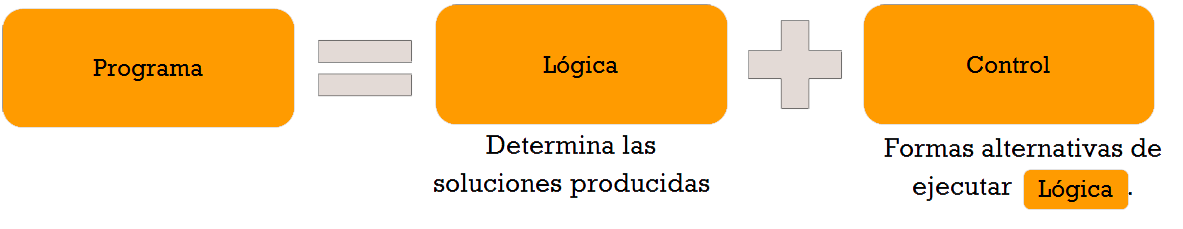
\includegraphics[scale=0.40]{./Imagenes/img02.png} 
\end{center}

Asume que partimos de un conjunto de hechos y reglas conocidos. Solamente es la declaración del componente lógico de un algoritmo. El sistema desarrolla el componente de control de secuencia. En este paradigma, la evaluación asume que cuando se selecciona una regla, es porque ésta es la única posibilidad o la necesaria para resolver el problema. Es decir, se encuentra una solución si un conjunto de reglas adecuado y las sustituciones a dichas reglas producen un conjunto de reglas aterrizadas (sin variables libres), suficientes para deducir el resultado de los hechos conocidos.
La programación lógica intenta resolver lo siguiente:
Dado un problema S, saber si la afirmación A es solución o no del problema o en que casos lo es. Además queremos que los métodos sean implantados en maquinas de forma que la resolución del problema se haga de forma automática
La programación lógica: construye base de conocimientos mediante reglas y hechos
\\
\\
Características
\\
\item Los programas para los lenguajes de programación lógicos son un conjunto de hechos y reglas.
\item La sintaxis de los lenguajes de programación lógicos es notablemente diferente de los lenguajes de programación imperativos.
\item	Unificación de términos.
\item	Mecanismos de inferencia automática.
\item	Recursión como estructura de control básica.
\item	Visión lógica de la computación.
\item	La aplicación de las reglas de la lógica para inferir conclusiones a partir de datos.
\item	El programa se transforma en un conjunto de declaraciones formales de especificaciones que deben ser correctas por definición.
\item	No tiene un algoritmo que indique los pasos que detallen la manera de llegar a un resultado.
\item	Las salidas son funcionalmente dependientes de las entradas.

Ventajas y Desventajas del uso de este paradigma
\\
Ventajas
\\

\item Puede mejorarse la eficiencia modificando el componente de control sin tener que modificar la lógica del algoritmo.
\item Relaciones multipropósito.
\item Simplicidad.
\item Generación rápida de prototipos e ideas complejas.
\item Sencillez en la implementación de estructuras complejas.
\item Potencia.
\\
Desventajas
\\
\item Altamente ineficiente.
\item Pocas áreas de aplicación
\item No existen herramientas de depuración efectivas.
\item En problemas reales, es poco utilizado.
\item Si el programa no contiene suficiente información para contestar una consulta responde false.
	

	
Ejemplo

De forma tradicional imperativa tendríamos que especificar como lo haremos

\begin{center}
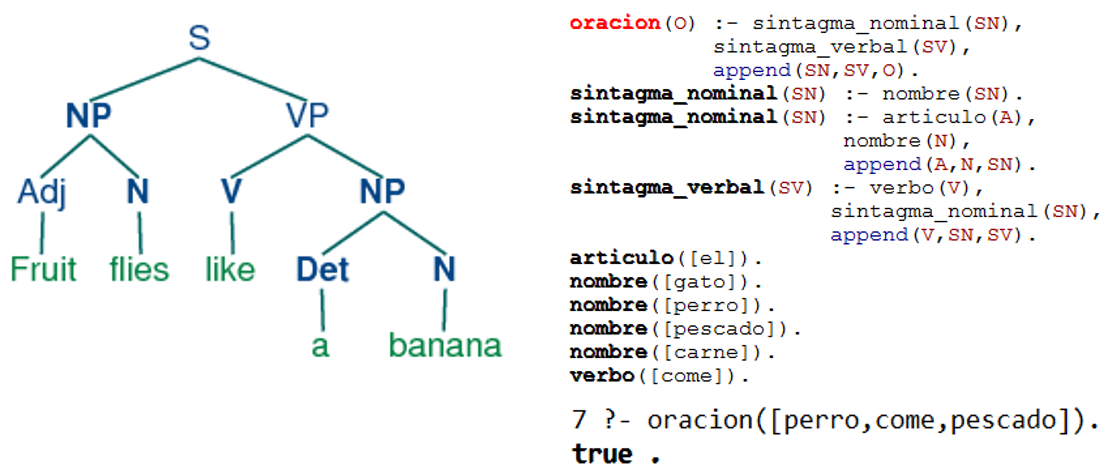
\includegraphics[scale=0.50]{./Imagenes/img08.png} 
\end{center}

Ejemplo
Un conjunto de hechos constituye un programa (la forma más simple de programa lógico) que puede ser visto como una base de datos que describe una situación. Por ejemplo, el Programa 1 refleja la base de datos de las relaciones familiares que se muestran en el siguiente gráfico.

\begin{center}
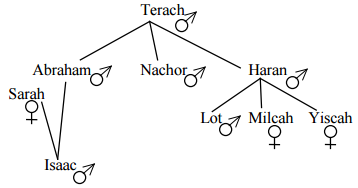
\includegraphics[scale=0.50]{./Imagenes/img09.png} 
\end{center}

\begin{center}
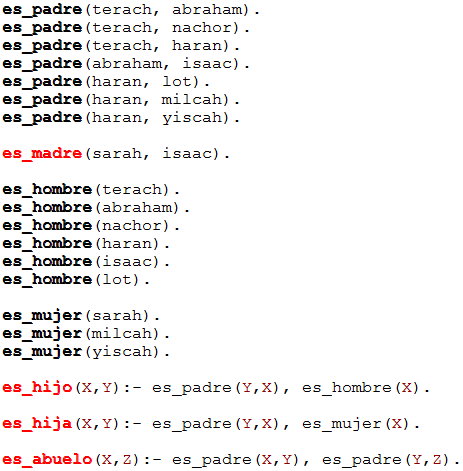
\includegraphics[scale=0.50]{./Imagenes/img10.png} 
\end{center}

\begin{center}
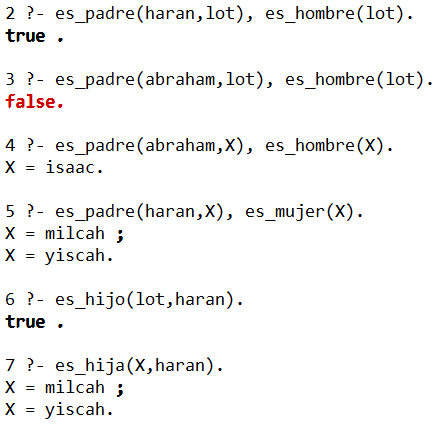
\includegraphics[scale=0.50]{./Imagenes/img11.png} 
\end{center}



\end{enumerate}





\section{Paradigma No 04 – Programación Funcional} 

\begin{enumerate}[1.]
	\item Programacion funcional:
\\
La Programación Funcional  es una forma en la cual podemos resolver diferentes problemáticas ya que estaremos trabajando principalmente con funciones, evitaremos los datos mutables, así como el hecho de compartir estados entre funciones.
\\	
\begin{center}
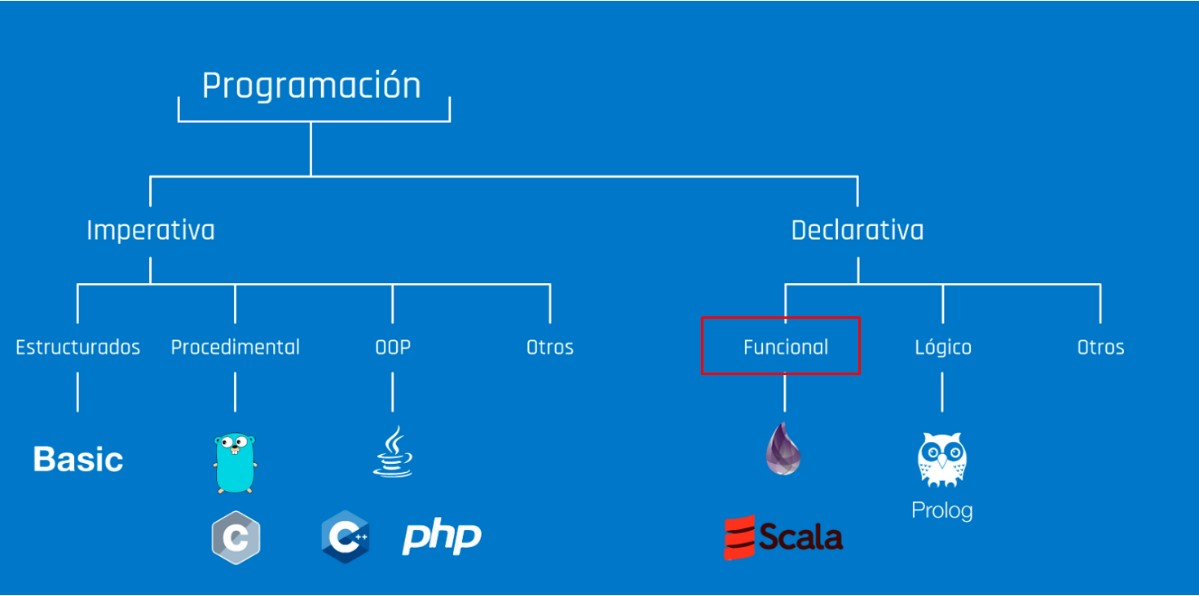
\includegraphics[scale=0.80]{./Imagenes/img04.jpg} 
\end{center}
Las funciones serán tratadas como ciudadanos de primera clase. Las funciones podrán ser asignadas a variables además podrán ser utilizadas como entrada y salida de otras funciones
\\
\\	
Ejemplo
\\
De forma tradicional imperativa tendríamos que especificar como lo haremos
\begin{center}
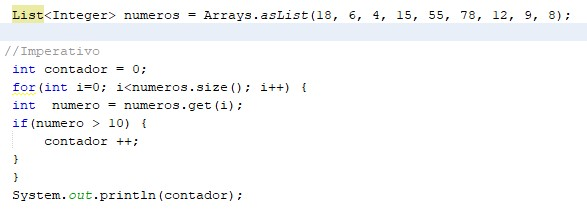
\includegraphics[scale=0.55]{./Imagenes/img05.jpg} 
\end{center}


Pero de forma declarativa o programación funcional tendríamos
\begin{center}
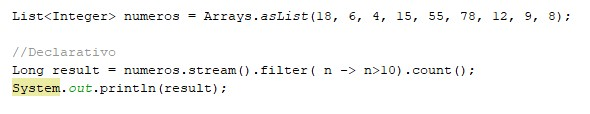
\includegraphics[scale=0.55]{./Imagenes/img06.jpg} 
\end{center}




\end{enumerate}






 
\include{Secciones/paradigma05}



\end{document}